\chapter{Q-Learning}\label{Ch:Q-Learning-Representations}

The previous chapter presented the backbone of Q-learning. In this chapter, we explain the details for implementing Q-learning algorithms. In section \ref{tabQ}, we demonstrate a tabular approach with the Cart Pole game as an example. The detailed results will appear in Chapter \ref{Ch:ResultsPrelim}. In section \ref{deepQ}, we explain the theoretical background for deep Q-learning. We introduce regularization in section \ref{reg}, which is the technique we used to improve our results in Chapter \ref{Ch:Analyze}.

\section{Tabular Q-Learning}\label{tabQ}
Having established the theoretical aspects of $Q$, it is necessary to find a 
suitable representation that can be found computationally. Two such 
representations will be discussed; here, a tabular representation is
described.

In the tabular setting, $Q$ will be represented by a look-up table where every
row corresponds to a state of the game and the respective columns represent
actions. Due to finite computational memory, storing the value of $Q$ for 
every possible state-action pair is infeasible when state spaces are continuous.
Consequently, continuous parameters from state spaces must be discretized into
disjoint bins. An example of such a discretization is given in Table 
\ref{table:disc_state_ex} for the game of Cart Pole.

\begin{table}[h!]
\centering
$\begin{aligned}[t]
x_t \in [-2.4, 2.4] &\Rightarrow {\{[-2.4, -0.8), [-0.8, 0.8), [0.8, 2.4]\}} \\
v_t^x \in [-\infty, \infty] &\Rightarrow {\{[-2, -1), [-1, 0),[0,1), [1, 2]\}}  \\
\theta_t \in [-0.419, 0.419] &\Rightarrow {\{[-0.419, -0.14), [-0.14, 0.14), [0.14, 0.419]\}}  \\
v_t^{\theta} \in [-\infty, \infty] &\Rightarrow {\{[-2, -1), [-1, 0), [0, 1), [1,2]\}} \\
\end{aligned}$
\caption[Discretized state space]{Since the state space is continuous, in order to represent the $Q$ function as a table, it is critical to discretize the state space.}
\label{table:disc_state_ex}
\end{table}

Once the state space has been discretized, each state can be mapped to its
corresponding bin which can then be mapped to a row in the tabular representation
of $Q$. An example of $Q$ for Cart Pole at some iteration is given in 
Table \ref{table: tab_q_ex}.

\begin{table}[h!]
\centering
\begin{tabular}{ c|c|c } 
  & Left & Right \\
 \hline
 {[1, 1, 1, 1]} & 0.8 & 0.3 \\
 {[1, 1, 1, 2]} &  & 0.6 \\
 \vdots & \vdots & \vdots \\
 {[2, 1, 2, 3]} & 0.15 & 0.11 \\
 \vdots & \vdots & \vdots \\
 {[3, 4, 3, 4]} & 1.2 & 0.9 \\
\end{tabular}
\caption[Tabular $Q$ example]{This table is an example of how to represent $Q$ function as a table. This table in particular stores the $Q$ function for the game Cart Pole, which was solved by the team. The details about solving Cart Pole is in Chapter \ref{Ch:ResultsPrelim}}
\label{table: tab_q_ex}
\end{table}

\subsection{Drawbacks}
While the tabular representation of $Q$ is favorable for pedagogical purposes and 
its implementation ease, it does not generalize well to games with large state 
spaces. For example, a gray-scale image with 1000 pixels has a state space size 
of $256^{1000}$. Storing values for each state is noticeably infeasible. Rather 
than storing the value of $Q$ for every possible state, we will use a function
to approximate $Q$. In particular, we will use a neural network to approximate
$Q$, as discussed in the next section.

\section{Deep Q-Learning}\label{deepQ}
\subsection{Overview}
In this section we outline the Deep Q-Learning (DQN) algorithm, which we took as the starting point 
of our investigation into Deep Reinforcement Learning. The basic idea of DQN is to represent the 
state-action value function Q as a convolutional neural network--recent work has shown deep neural networks to work
well in this setting. 

There are three simple modifications one has to make to the tabular Q-Learning algorithm to get what 
is now commonly called the DQN-algorithm \cite{mnih2013playing}. We outline these modifications below. 

\subsection{Q as a neural network}
The first step is to replace the function $Q:S\times A \rightarrow \mathbb{R}$ by a neural network \linebreak
${Q(\cdot, \cdot \mid \theta):S \times A \rightarrow \mathbb{R}}$, where $\theta$ denotes the weights of the model.
The resulting network, called 
the Q-network, takes as its input a state and an action, and outputs the estimated Q-value of the 
pair. But the question arises: How do we find good parameters $\theta$ for this model? Suppose that
 at timestep $i$ we have current estimates $\theta_i$ for the weights of the network. We take the loss function to be the mean squared TD-error, the same error term as used in the simple 
 tabular Q-learning algorithm, derived from the Bellman optimality equation. 
\begin{align}
L_i(\theta_i) = \mathbb{E} \left[ \left( \E\left.\left[ R_{t+1} + \gamma\, \max\limits_{a'} Q(s_{t+1}, a' \mid \theta_{i-1}) \right| s_t, a_t \right] - Q(s_t, a_t \mid \theta_i) \right)^2 \right]
\end{align}

Because the dynamics of the environment the agent is operating in is unknown, the expectation above cannot be evaluated;
we get around this by using Stochastic
Gradient Descent (SGD). Using this method,
we get the following update rule for the weights $\theta$ :
\begin{align}
\nabla_{\theta_i} L_i (\theta_i) &= \mathbb{E} \left[ \left(R_{t+1} + \gamma\, \max\limits_{a'} Q(s_{t+1}, a' \mid \theta_{i-1}) - Q(s_t, a_t \mid \theta_i) \right) \nabla_{\theta_i} Q(s_t, a_t \mid \theta_i ) \right] \\
\theta_{i+1} &= \theta_i - \alpha\, \nabla_{\theta_i} L_i (\theta_i) \rvert _{\theta_i}
\end{align}

\subsection{Experience Replay and Fixed Q-Targets}
In theory, SGD only works under some independence assumptions on the data 
we feed it. We need to ask ourselves whether these assumptions are reasonable in this setting. As 
we are playing the game, and updating our weights at each timestep, the sequence of transitions 
visited by the agent is highly correlated: We cannot reasonably expect the game's state to be independent
of its immediate past. Therefore, we use the method of experience replay to decorrelate the data and  
to achieve higher data efficiency. Moreover, this helps 
reduce the risk of getting stuck  in unwanted feedback loops. 

At each timestep, we store the tuple $(s_t, a_t, R_{t+1}, s_{t+1})$ in the replay memory denoted by 
$\mathcal{D}$. Instead of updating $\theta$ based on the most recent transition, we instead sample 
uniformly from $\mathcal{D}$, and use these past experiences to perform the gradient descent step. 
In practice, we sample a minibatch of transitions $(s_j, a_j, R_{j+1}, s_{j+1})_{j \in J}$ where the 
minibatch size $|J|$ is usually chosen to be a multiple of 2 in the range of 16 to 64. This way we reuse all experiences
 multiple times during training. Another parameter that arises from experience replay is the replay 
 memory capacity - the maximum length of the replay memory - which is chosen in the range of $10^3$ to $10^6$.

The final modification that needs to be made in order for DQN to work is the method of fixed Q-targets. 
In the loss function, in the absence of supervision, one must bootstrap from the current weights $\theta_i$ 
in order to arrive at the TD-error, an estimate of Q's accuracy. However, instead of using the most recent 
estimates $\theta_i$, one can use a separate, periodically updated set of weights, usually denoted by $\theta^-$. 
After the modification, the loss function becomes 
\begin{align}
L_i(\theta) = \mathbb{E} \left[ \left( \E\left.\left[ R_{t+1} + \gamma\, \max\limits_{a'} Q(s_{t+1}, a' \mid {\color{red} \theta^-}) \right| s_t, a_t \right] - Q(s_t, a_t \mid \theta) \right)^2 \right]
\end{align}

\begin{figure}[h!]
\centering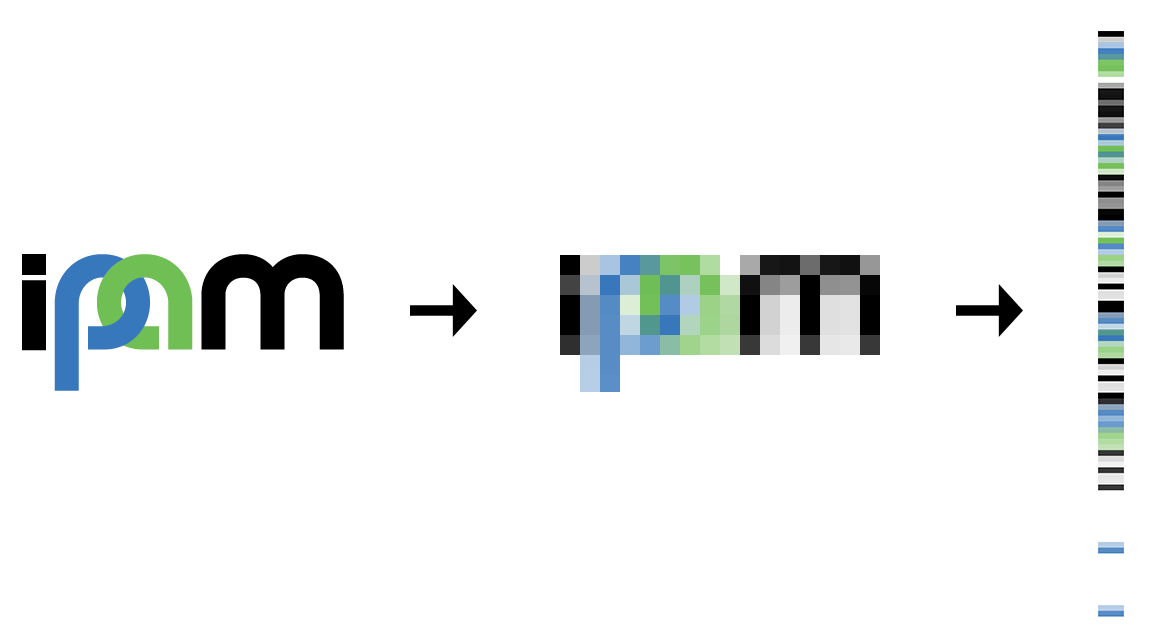
\includegraphics[scale=0.25,clip]{Graphics/ipam.png}
\caption[Downsampling and Flattening the Logo of IPAM]{This is an illustration of the pre-processing method commonly employed in RL algorithms.}
\label{fig:ipam}
\end{figure}

\newpage
\section{Q-learning in practice}
We now address the question of how the data used to train
the agent is generated. In practice, $Q$ is initialized randomly, thus immediately taking the actions suggested
by $Q$ as in Equation (\ref{eq:q_iter_up}) will introduce bias towards the 
initialization of $Q$. As such, the agent is expected to explore the state space 
and determine which actions are more suitable for certain states. Consequently,
a parameter $\epsilon \in [0,1]$ will be used to determine which action to take
at each iteration: with probability $\epsilon$, a random action will be taken; 
with probability $1 - \epsilon$ the action suggested by $Q$ will be taken. In more complex computer games, the only observation the agent is given 
by its environment is an RGB image of the screen for each frame of the game. We process these images, 
in order to be able to use them as input to the Q-network. We do so following the methods used by Mnih et al. in \textit{Playing Atari with Deep Reinforcement Learning} \cite{mnih2013playing}:
at each timestep, we take the most recent four frames, convert them to grayscale, downsample to a size 
of $84\times 84$, and then stack them to produce the input to the network. A toy visualization of this process is given in
Figure \ref{fig:ipam}.

\section{Regularization}\label{reg}
A common problem among machine learning algorithms is 
that the algorithm often overfits to the training data 
and struggles to generalize to new inputs during testing. 
Many strategies have been developed to address this, possibly at the expense of increasing the training 
error. These strategies are collectively called regularization. 
\par
In deep learning, most regularization strategies are based on 
regularizing estimators, such as parameter norm penalties where 
parameters are penalized based on its norm. In other words, the 
larger the effect a parameter has on the outcome, the more heavily 
the parameter will be penalized, forcing the algorithm to not 
overfit to certain features during training. 
\par
In our project, we chose \textbf{dropout} as our regularization method as
it provides a computationally inexpensive method for 
regularizing the models. The next section expands on the
theoretical aspects of dropout.

\subsection{Dropout}
Dropout was first introduced by Srivastava et al. in 2014 
\cite{JMLR:v15:srivastava14a} as a regularization method. Dropout 
drops units (along with their connections) from the neural 
network during training, preventing estimators from 
co-adapting to the training samples. Alternatively, dropout can be understood in the context of bagging. In particular, dropout separates a large neural network
into an ensemble of of many sub-networks, which is similar to bagging. Bagging involves training multiple models and evaluating multiple models for each test case. However, bagging becomes impractical when it comes to large neural networks due to the huge amount of training time and computational power required. Dropout provides a way to implement bagging on large neural networks since it essentially trains sub-networks at once and infers the results from the collective knowledge of all sub-networks.

\begin{figure}[h!]
\centering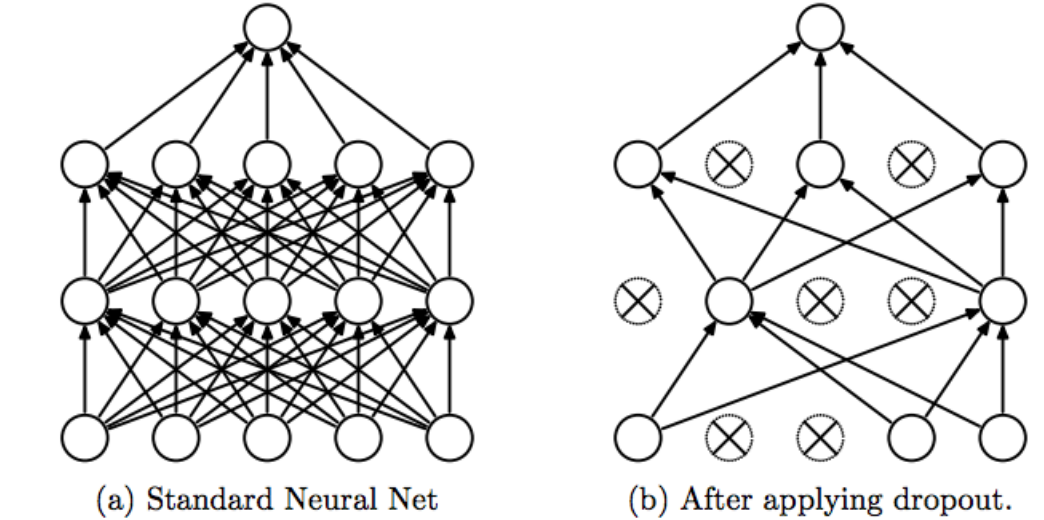
\includegraphics[scale=0.3,clip]{Graphics/dropout.png}
\caption[Illustration of Dropout]{This figure shows how dropout decomposes a connect neural network into sub-networks. The cross marks on neurons indicate that the neurons are zeroed out and not included in the sub-network.}
\label{fig:dropout}
\end{figure}

Dropout seeks to divide a large neural network into sub-networks by `dropping out' some of the neurons in the network. During training, a mask containing zeros and ones is randomly generated based on a hyperparameter for determining the percentage of neurons to keep in the sub-networks. This mask is then applied to the neural network, zeroing the weights of some neurons. By performing this operation, a large neural network is decomposed into sub-networks. During inference, the result is calculated based on the geometric mean of the results from all sub-models given by
\begin{align}
\tilde{p}_{ensemble}(y | \boldsymbol{x})=\sqrt[2^d]{\prod_{\boldsymbol{\mu}} p(y | \boldsymbol{x},\boldsymbol{\mu})}
\end{align}

where $\boldsymbol{\mu}$ is the randomly generated mask, d is the number of neurons that may be dropped, $\boldsymbol{x}$ is the input and $y$ is the predicted output.
\par
After taking the geometric mean, it is necessary to normalize the ensemble:
\begin{align}
p_{ensemble}(y | \boldsymbol{x})=\frac{\tilde{p}_{ensemble}(y | \boldsymbol{x})}{\sum_{y'} \tilde{p}_{ensemble}(y' | \boldsymbol{x})}
\end{align}

Dropout is a commonly used regularization method in deep neural networks. It is commonly believed that dropout is not necessary for deep RL algorithms because overfitting does not occur often in the RL realm. Due to the large state space, it is not likely for the model to overfit to the environment. However, we provide an counter example in Chapter \ref{Ch:Analyze} to demonstrate that the use of dropout could improve performance and save training time by generalizing model trained in a fixed environment.


\endinput

